\newpage
\section{Określenie wymagań szczegółowych}		%2
%Dokładne określenie wymagań aplikacji (cel, zakres, dane wejściowe) – np. opisać przyciski, czujniki, wygląd layautu, wyświetlenie okienek. Opisać zachowanie aplikacji – co po kliknięciu, zdarzenia automatyczne. Opisać możliwość dalszego rozwoju oprogramowania. Opisać zachowania aplikacji w niepożądanych sytuacjach.

\subsection{Cel aplikacji}
Celem aplikacji jest ułatwienie studentom oraz pracownikom uczelni dostępu do kluczowych funkcji administracyjnych i informacyjnych związanych z edukacją. Aplikacja ma zastąpić tradycyjne interakcje z dziekanatem, umożliwiając szybki dostęp do ocen, planu zajęć, harmonogramu egzaminów, czy otrzymywania powiadomień.

\begin{itemize}
      \item \textbf{Zakres aplikacji:}
            \\\textbf{Studenci}: dostęp do ocen, planu zajęć, harmonogramu egzaminów, powiadomień.
            \\\textbf{Administracja: }zarządzanie danymi, kontakt ze studentami.
      \item \textbf{Platformy:}
            \\\textbf{Systemy operacyjne:} \\Android, \\iOS.
      \item \textbf{Dane wejściowe: (Logowanie użytkowników)}
            \\\textbf{Dane studentów}: nr indeksu, rocznik, oceny, plan zajęć, egzaminów, zgłoszenia do dziekanatu.
            \\\textbf{Zdarzenia dziekanatu}: zmiany w planie, ogłoszenia, nowe dokumenty, powiadomienia o ocenach.
      \item \textbf{Opis interfejsu użytkownika i elementów interaktywnych:}
            \newpage
            \textbf{Ekran logowania:  Rys. \ref{rys:ekranlogowania} (s. \pageref{rys:ekranlogowania})}
            \begin{figure}[htb!]
                  \centering
                  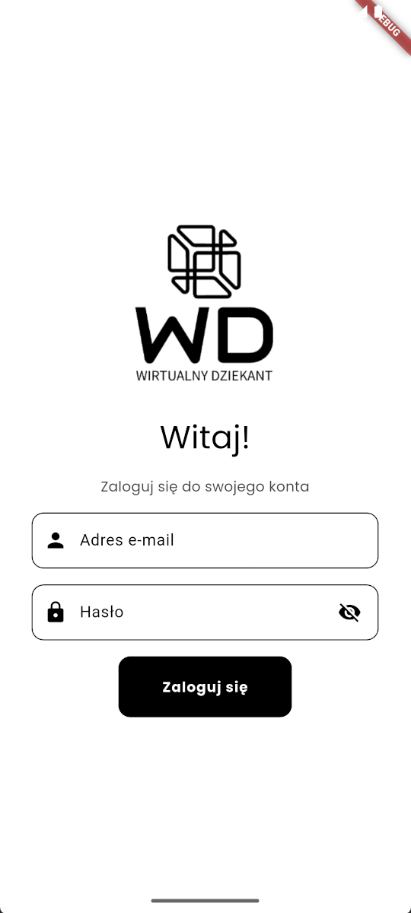
\includegraphics[width=0.65\linewidth]{rys/ekranlogowania.png}
                  \caption{Ekran logowania}
                  \label{rys:ekranlogowania}
            \end{figure}
            \newpage
            \textbf{Pola tekstowe:} „Email” oraz „Hasło”.
            \\\textbf{Przyciski:} „Zaloguj” – po kliknięciu, autoryzacja danych w tle i przejście do ekranu głównego. W przypadku błędnych danych, komunikat „Niepoprawne dane logowania”. „Zapomniałem hasła” – przekierowanie do formularza resetowania hasła.
      \item  \textbf{Ekran główny (Dashboard): Rys. \ref{rys:ekranglowny} (s. \pageref{rys:ekranglowny})}
            \begin{figure}[htb!]
                  \centering
                  
\includegraphics[width=0.8\linewidth]{rys/ekranglowny.png}
                  \caption{Ekran główny}
                  \label{rys:ekranglowny}
            \end{figure}
            \\Wyświetlane informacje: skrót do ocen, nadchodzących zajęć, powiadomienia o ważnych wydarzeniach.
            \\\textbf{Przyciski:}
            \\\textbf{„Przedmioty”} – po kliknięciu, przejście do ekranu z listą ocen, harmonogramu egzaminów z możliwością filtrowania według przedmiotu.
            \\\textbf{„Plan zajęć”} – po kliknięciu, podgląd planu zajęć (interaktywny kalendarz).
            \\\textbf{„Ustawienia”} – po kliknięciu, przejście do ustawień naszego profilu
            \\\textbf{Automatyczne zdarzenia}: wyświetlanie powiadomień push o nadchodzących zajęciach, ocenach, ważnych wydarzeniach.
            \newpage
      \item \textbf{Ekran ocen:  Rys. \ref{rys:ekranocen} (s. \pageref{rys:ekranocen})}
            \begin{figure}[htb!]
                  \centering
                  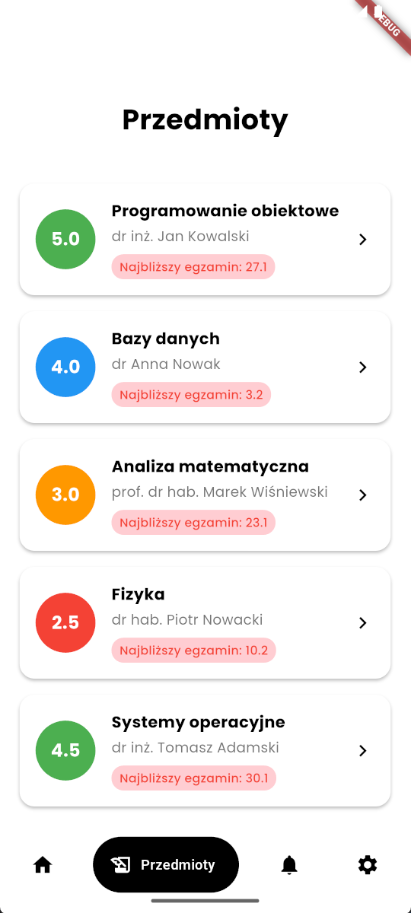
\includegraphics[width=0.65\linewidth]{rys/ekranocen.png}
                  \caption{Ekran ocen}
                  \label{rys:ekranocen}
            \end{figure}
            \newpage
            \textbf{Tabela ocen:} kolumny „Przedmiot”, „Ocena”, „Komentarz wykładowcy”, „Data”.
            \\\textbf{Opcje sortowania}: sortowanie ocen po przedmiocie, dacie.
            \\\textbf{Zachowanie:} po kliknięciu w przedmiot, otwarcie szczegółów przedmiotu (np. opis, prowadzący, historia ocen).
            Plan zajęć:

      \item \textbf{Widok kalendarza}: wyświetlanie zajęć na dany tydzień/dzień.
            \\\textbf{Funkcje interaktywne Rys. \ref{rys:ekranplanzajec} (s. \pageref{rys:ekranplanzajec})}:
            \begin{figure}[htb!]
                  \centering
                  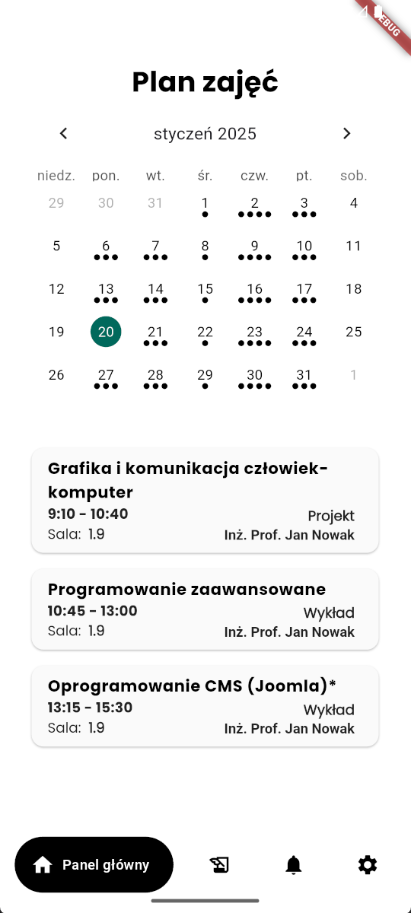
\includegraphics[width=0.55\linewidth]{rys/ekranplanzajec.png}
                  \caption{Ekran Planu zajęć}
                  \label{rys:ekranplanzajec}
            \end{figure}
            \newpage
            Zmiana tygodnia za pomocą przesuwania palcem (swipe left/right).
            \\Kliknięcie na zajęcia otwiera szczegóły, np. nazwisko wykładowcy, sala, godziny.
            \\Powiadomienia push: automatyczne przypomnienia o nadchodzących zajęciach z możliwością wyłączenia.

      \item \textbf{Harmonogram egzaminów Rys. \ref{rys:ekranegzaminow} (s. \pageref{rys:ekranegzaminow})}:
            \begin{figure}[htb!]
                  \centering
                  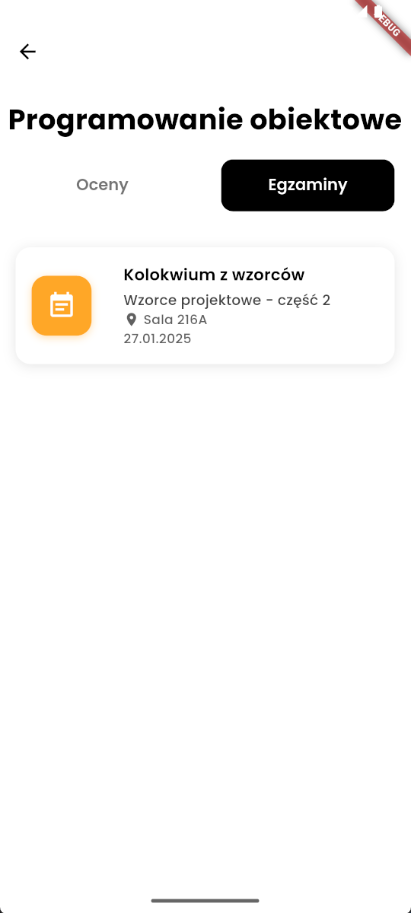
\includegraphics[width=0.55\linewidth]{rys/ekranegzaminow.png}
                  \caption{Ekran Egzaminów}
                  \label{rys:ekranegzaminow}
            \end{figure}
            \newpage
            \textbf{Lista egzaminów}: możliwość filtrowania według przedmiotu, prowadzącego, daty.
            \\\textbf{Powiadomienia push}: przypomnienia o zbliżających się egzaminach.
            Komunikacja z dziekanatem:

      \item \textbf{Zdarzenia automatyczne}:
            \\Aplikacja będzie automatycznie wysyłać powiadomienia push o zmianach w planie zajęć, wynikach egzaminów, nowo dodanych dokumentach i ogłoszeniach.
            \\Automatyczne aktualizacje planu zajęć oraz harmonogramu egzaminów po synchronizacji z serwerem (np. co 30 minut).
      \item \textbf{Działanie offline}:
            \\Gdy brak połączenia z internetem, użytkownik ma dostęp do zapisanych wcześniej danych (plan zajęć, oceny).
      \item \textbf{Zachowanie aplikacji w niepożądanych sytuacjach}:
            \\\textbf{Brak połączenia z internetem:}
            \\Aplikacja wyświetla komunikat „Brak połączenia. Sprawdź połączenie z internetem” przy próbie wykonania operacji wymagającej synchronizacji z serwerem (np. wysłanie wiadomości do dziekanatu).
            W trybie offline: dostęp do zapisanych danych, brak możliwości interakcji z funkcjami wymagającymi połączenia.
            \\\textbf{Błędne dane logowania}:
            \\Komunikat „Niepoprawny email lub hasło” oraz możliwość ponownego wpisania danych. Pole tekstowe zostaje podświetlone na czerwono.
            \\\textbf{Serwer niedostępny}:
            \\Wyświetlenie komunikatu „Serwer dziekanatu jest obecnie niedostępny. Spróbuj ponownie później”.
            \\\textbf{Niepoprawne działanie aplikacji}:
            \\W przypadku błędu technicznego aplikacja wyświetli komunikat „Wystąpił błąd. Spróbuj ponownie” i zapisze logi błędów do późniejszej analizy przez programistów.
\end{itemize}
